\documentclass{article}
\usepackage{ctex}
\usepackage{graphicx}
\usepackage{amsfonts}
\usepackage{amsmath}
\usepackage{subfig}
\usepackage{listings}
\usepackage{xcolor}
\usepackage{pythonhighlight}
\usepackage
[a4paper,
text={146.4true mm,239.2 true mm},
top= 26.2true mm,
left=31.8 true mm,
head=6true mm,
headsep=6.5true mm,
foot=16.5true mm]
{geometry} % 设置文本的边距
\setlength{\parskip}{1.0em}


\begin{document}
    \title{基于DQN算法的平衡小车控制}
    \author{姓名:林奇峰$\quad$学号:19110977}
    \date{}
    \maketitle

    \section{摘要}
        平衡小车的控制问题(CartPole)是一个经典的强化学习问题。本文利用DQN算法来控制平衡小车的移动使其上面的杆维持竖直的状态。实验结果表明DQN算法可以学习到平衡小车的控制策略。本文也对训练过程中出现的现象和问题进行了分析,并认为DQN算法可以对连续状态空间进行一定的放大来获得比较好的效果。
    \section{引言}
        平衡小车的控制问题是一个经典的强化学习问题。在这个问题中,平衡小车上面的杆需要在小车移动的过程中保持竖直的状态,而小车的移动方向会影响杆的倾斜方向。因此,一个好的策略需要不断地控制小车的移动方向来使得杆保持竖直,如图\ref{fig:cartpole}所示:
        \begin{figure}[h]
            \centering
            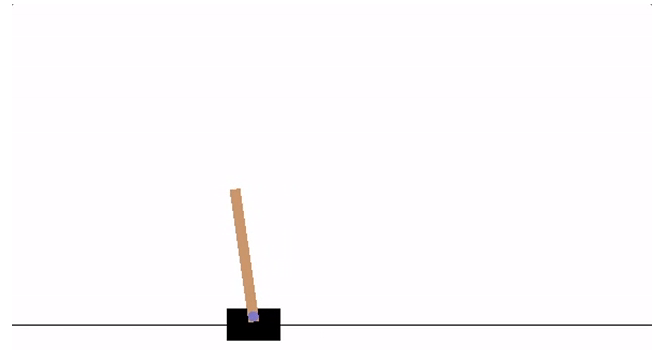
\includegraphics[width=3.0in]{cartpole.png}
            \caption{CartPole示例}
            \label{fig:cartpole}
        \end{figure}

        CartPole问题可以建模成一个马尔可夫决策问题(Markov Process Decision,简称MDP),因为控制小车的移动方向只与当前状态有关,与更早之前的状态和决策无关。

        当前深度强化学习算法在许多应用上面获得了很多的成功,如DQN算法。因此本文研究了DQN算法在CartPole问题上的应用,并对训练过程进行了分析。实验结果表明DQN算法可以完成CartPole任务,且可以通过放大连续的状态向量来达到比较好的效果。
    \section{方法}
        强化学习是基于MDP框架的一类算法。MDP可以用四元组$<S,A,T,r>$表示。其中$S$代表有限的状态集合,$A$代表动作空间,$T:S\times A\rightarrow S$代表状态转移函数,$r:S\times A\rightarrow\mathbb{R}$代表即时奖励。

        DQN算法是结合了经典的强化学习算法和深度学习算法。其方法主要是最小化TD error:
        \begin{equation}
            \delta_t = r_t+\gamma Q'(s_{t+1}, a_{t+1})-Q(s_t,a_t)
        \end{equation}
        其中$t$代表时间戳,$\gamma$为折扣因子。$Q$函数是采用神经网络近似,为在线网络,而$Q'$函数需要每隔一段时间用$Q$函数的参数进行更新,为目标网络。因此,损失函数的公式为:
        \begin{equation}
            \mathcal{L}=[r+\gamma Q'(s',a')-Q(s,a)]^2
        \end{equation}
        
        另外,DQN算法还采用了回放经验池$\mathcal{D}$(Experience Replay Buffer)的方法来稳定训练过程。$\mathcal{D}$中的每个元素为四元组$(s,a,s',r)$。
    \section{实验}
        实验采用了gym库中的CartPole-V0环境。其中状态表示为长度为4的向量,里面的元素分别为推车位置$[-2.4, 2.4]$,车速$[-\infty, \infty]$,杆子角度$[-41.8, 41.8]$与杆子末端速度$[-\infty, \infty]$。动作空间只有向左和向右,分别用0和1表示。每一步的移动都会得到+1的奖励。当连续100个episode的平均累积奖励超过195的时候,CartPole问题就可以被视为解决了。

        \subsection{实验一:DQN算法在CartPole上的初步实验}
        实验参数表 \ref{table:parameter1}所示。其中lr为学习率,num\_hidden为隐层神经元个数,batch\_size为一次训练使用的样本数量,max\_size为回放经验池的最大容量,gamma为折扣因子,而rate为目标网络的更新速率。更新的公式为:
        \begin{equation}
            \theta' = rate * \theta + (1-rate) * \theta'
        \end{equation}
        \begin{table}[h]
            \centering
            \begin{tabular}{c|c|c|c|c|c}
                \hline
                lr & num\_hidden & batch\_size & max\_size & gamma & rate\\
                \hline
                1e-4 & 12 & 100 & 1e6 & 0.9 & 1e-3\\
                \hline
            \end{tabular}
            \caption{实验一参数设置}
            \label{table:parameter1}
        \end{table}

        实验一共运行了20000个episode。实验取每100个Episode的值的平均值作为实验结果,如图\ref{fig:reward}-\ref{fig:dcw}所示。

        图\ref{fig:reward}为奖励曲线,纵轴的数值为连续100个Episode的平均奖励。从曲线的上升趋势中我们可以看到DQN算法可以逐渐学习到比较好的策略来逐渐提高表现。

        图\ref{fig:loss}为损失函数曲线,纵轴的数值为进行开根号并对数处理后的损失函数数值。可以看到随着训练的进行,损失函数逐渐减小,而TD error也逐渐减小。这也符合直观的训练过程理解。

        \begin{figure}[htb]
            \centering
            \subfloat[奖励曲线]{
                \label{fig:reward}
            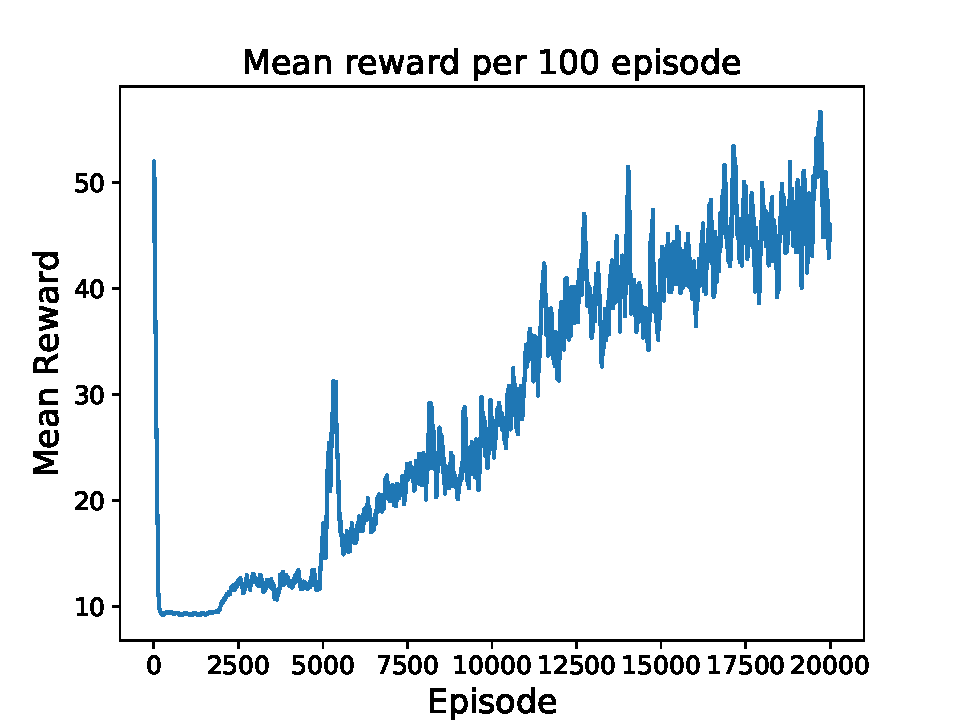
\includegraphics[width=2.5in]{episode.pdf}
            }
            \subfloat[损失函数曲线]{
                \label{fig:loss}
                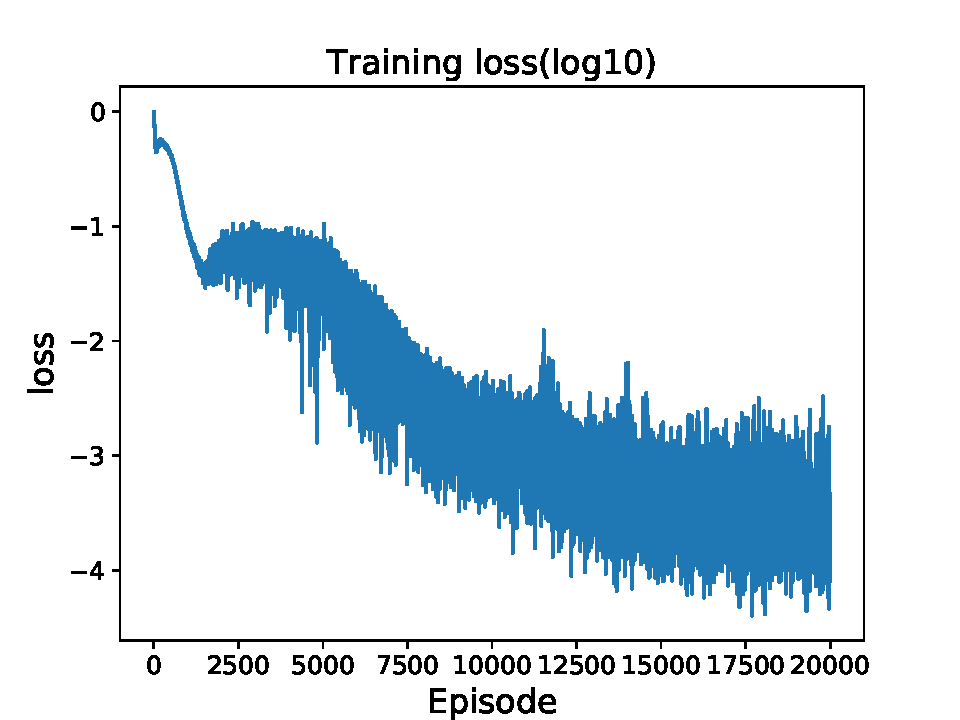
\includegraphics[width=2.5in]{loss.pdf}
            }
            \caption{奖励曲线和损失函数曲线}
        \end{figure}
        
        图\ref{fig:cn}为当前$Q$值与下一步的$Q$值曲线图。首先,我们可以看到两者的曲线都在向上提升。这符合我们一开始的直观理解。因为DQN应该会引导智能体不断地选择Q值增大的方向学习。其次,我们可以看到$Q$和$Q'$的数值上很接近。按照一开始的理解,两者之间应该存在着近似1的差别。其实,一开始的时候,两者确实存在着近似1的差别。但随着训练的进行,两者越来越接近。我们把两者之间的差取对数以后可以得到图\ref{fig:dcn}的结果。可以看到,一开始两者之间的确是存在接近1的差别,但是后面就逐渐减小差别。这应该是归结于状态空间为连续空间。连续空间的变化可能不够剧烈和明显,从而导致DQN的数值变化也不明显。
        \begin{figure}[htb]
            \centering
            \subfloat[当前Q值与下一步的Q值曲线]{
                \label{fig:cn}
                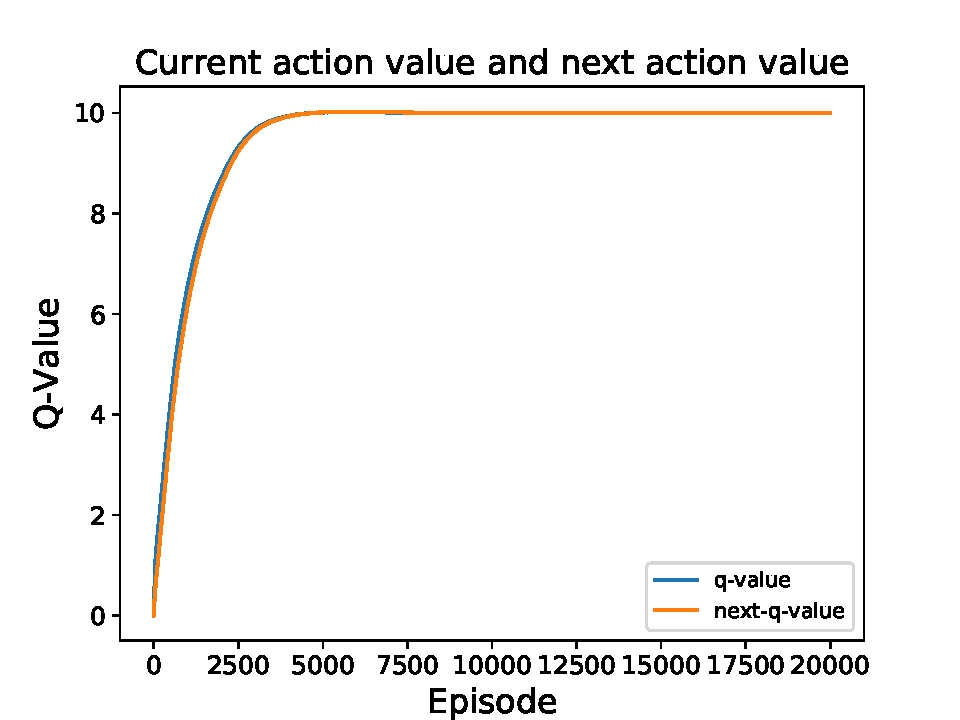
\includegraphics[width=2.5in]{cn.pdf}
            }
            \subfloat[当前Q值与下一步的Q值之差的曲线]{
                \label{fig:dcn}
                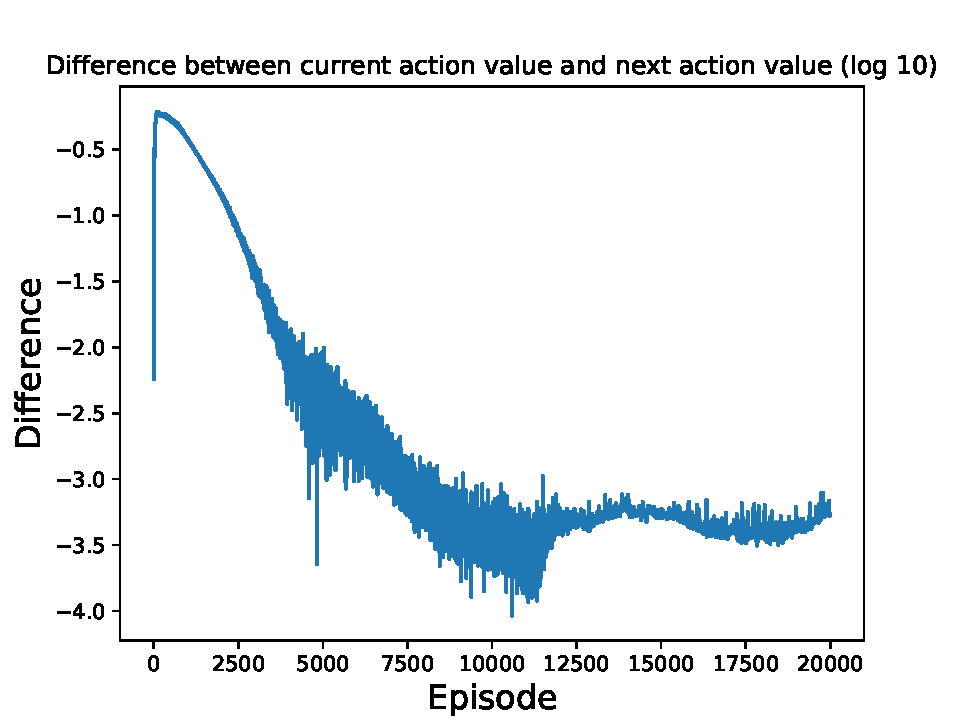
\includegraphics[width=2.5in]{dcn.pdf}
            }
            \caption{当前Q值与下一步的Q值的相关曲线}
        \end{figure}

        图\ref{fig:cw}为每一步正确动作和错误动作之间的Q值曲线。首先,正确动作的Q值曲线会上升比较符合直观的理解,但是错误动作的Q值曲线应该会一直下降,而实验结果却有点出乎我的意料。我们可以看到两者之间的曲线在数值上也是非常接近的。为了更好地分析其中的变化,我们将两者之间的差进行了对数处理得到图\ref{fig:dcw}。可以看到一开始两者之间的差别是拉大的,但是随着训练的进行,两者之间的差别又缩小。这应该还是因为连续的状态空间导致变化对DQN算法来说不够明显和易于区别。     
        \begin{figure}[htb]
            \centering
            \subfloat[正确动作与错误动作的Q值曲线]{
                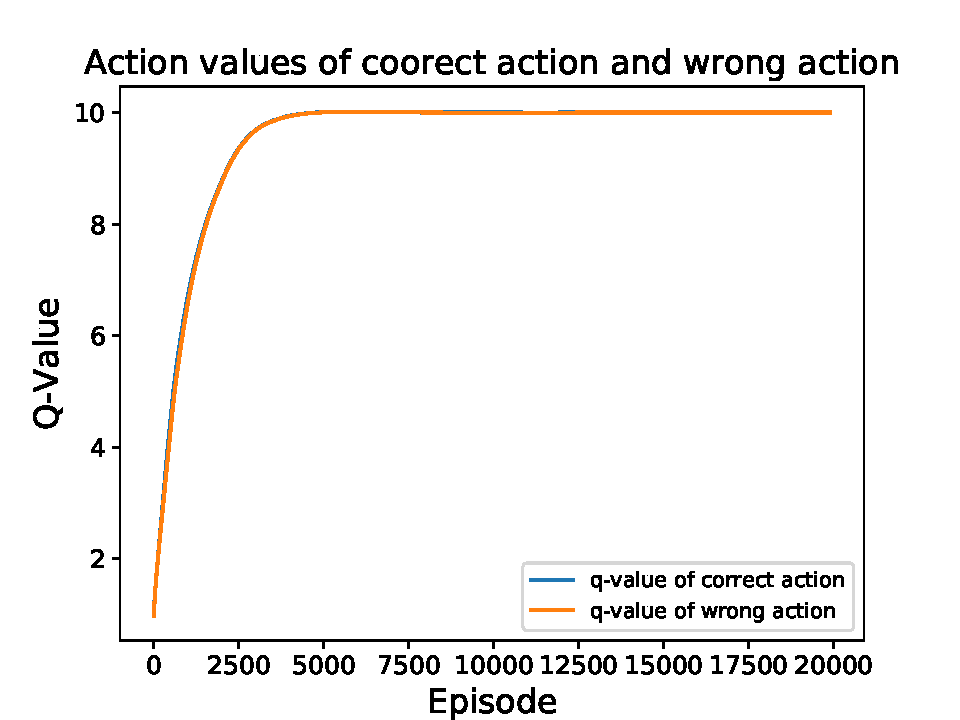
\includegraphics[width=2.5in]{cw.pdf}
                \label{fig:cw}
            }
            \subfloat[正确动作与错误动作的Q值之差的曲线]{
                \label{fig:dcw}
                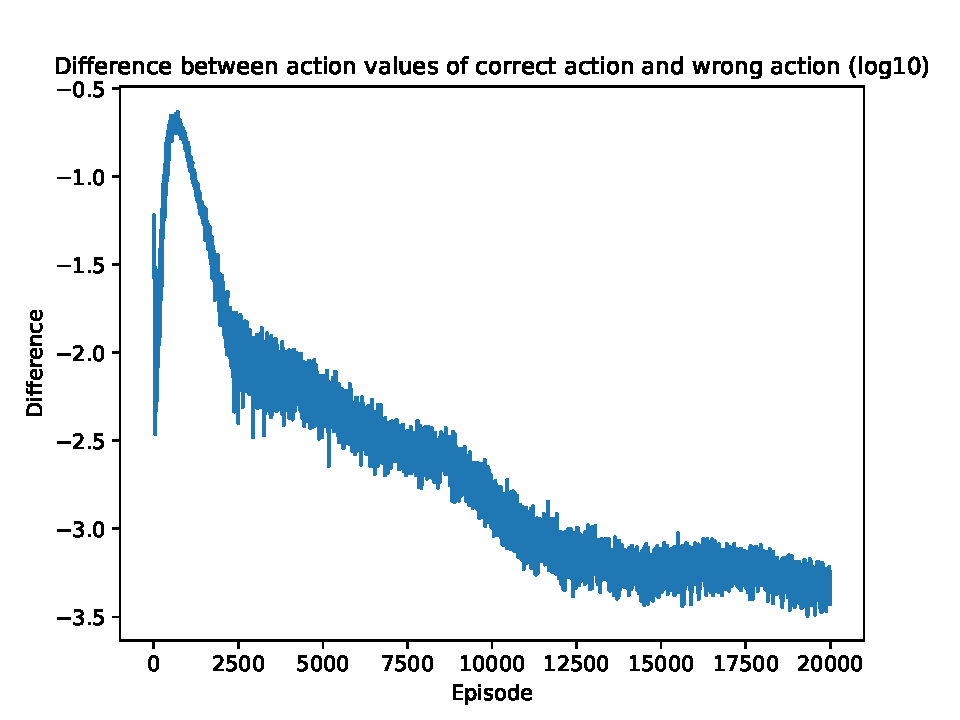
\includegraphics[width=2.5in]{dcw.pdf}
            }       
            \caption{正确动作与错误动作的Q值相关曲线}
        \end{figure}

        从上述结果我们可以看到对连续状态空间来说,我们可能需要对其变化进行一定的放大来使得状态之间的区分度更高一点。
        
        \subsection{实验二:状态放大对于DQN算法的影响}
        为了验证变化放大的分析,我对状态向量的数值乘上一个缩放因子scale。上述实验一的结果可以看成设置为scale=1.0的结果。下面给出scale=16.0的结果。
        实验参数如表\ref{table:parameter2}所示:
        \begin{table}[h]
            \centering
            \begin{tabular}{c|c|c|c|c|c}
                \hline
                lr & num\_hidden & batch\_size & max\_size & gamma & rate\\
                \hline
                1e-5 & 10 & 100 & 1e6 & 0.9 & 1e-3\\
                \hline
            \end{tabular}
            \caption{实验二参数设置}
            \label{table:parameter2}
        \end{table}

        本次实验只需要运行2000个episode。实验结果如图\ref{fig:reward2}-\ref{fig:dcw2}所示。从图\ref{fig:reward2}可以看到经过状态放大,我们可以在2000个episode以内完成CartPole任务。但是DQN算法会存在过拟合的问题,需要一定的停止策略。从图\ref{fig:cn2}和\ref{fig:dcn2}中我们可以看到训练的后期前后两步的Q值依然会逐渐缩小差距。这可能也是DQN算法过拟合的原因。从图\ref{fig:cw2}和\ref{fig:dcw2}中,我们可以看到一开始正确动作和错误动作的差距会扩大,然后差距缩小到一定的地步的时候DQN算法会有比较好的结果。但是在训练后期由于过拟合两者的差距又会缩小。所以我们可以考虑在两者之间的差距开始缩写的时候停止DQN算法的训练。


        因此,上述结果说明对于连续状态空间,进行程度的状态放大确实可以提高DQN算法的效果和减少训练时间。
        \begin{figure}[htb]
            \centering
            \subfloat[奖励曲线]{
                \label{fig:reward2}
            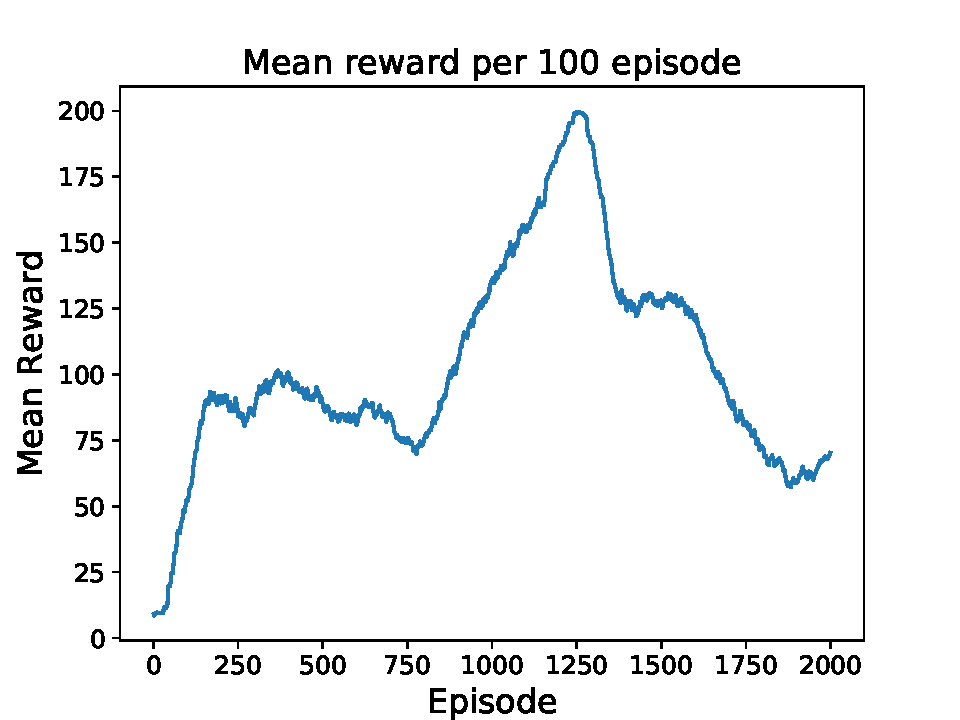
\includegraphics[width=2.5in]{episode2.pdf}
            }
            \subfloat[损失函数曲线]{
                \label{fig:loss2}
                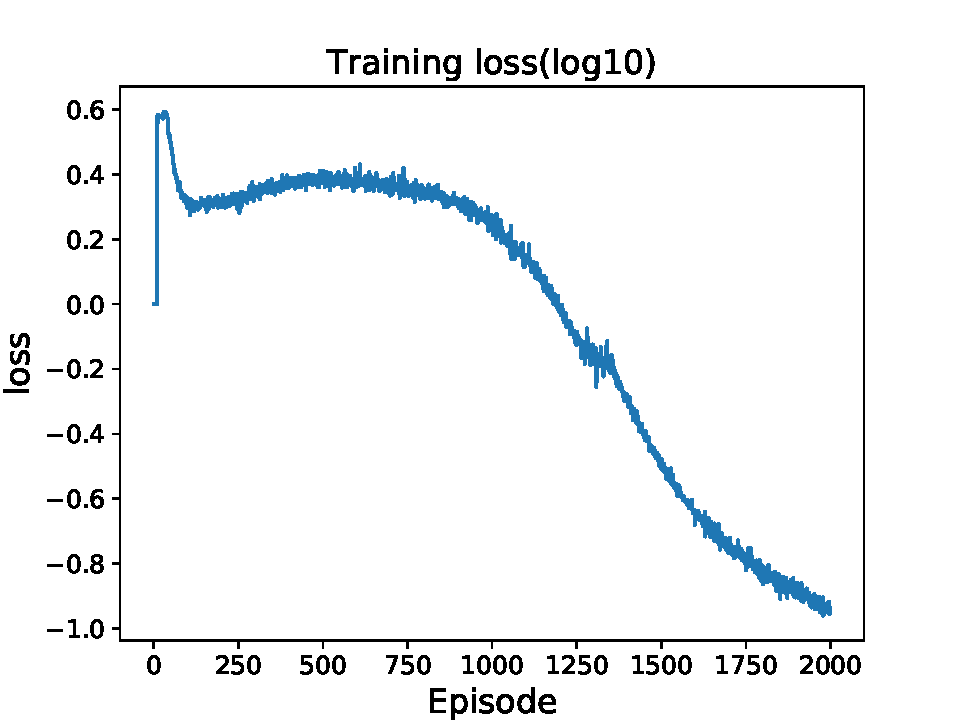
\includegraphics[width=2.5in]{loss2.pdf}
            }
            \caption{奖励曲线和损失函数曲线}
        \end{figure}

        \begin{figure}[htb]
            \centering
            \subfloat[当前Q值与下一步的Q值曲线]{
                \label{fig:cn2}
                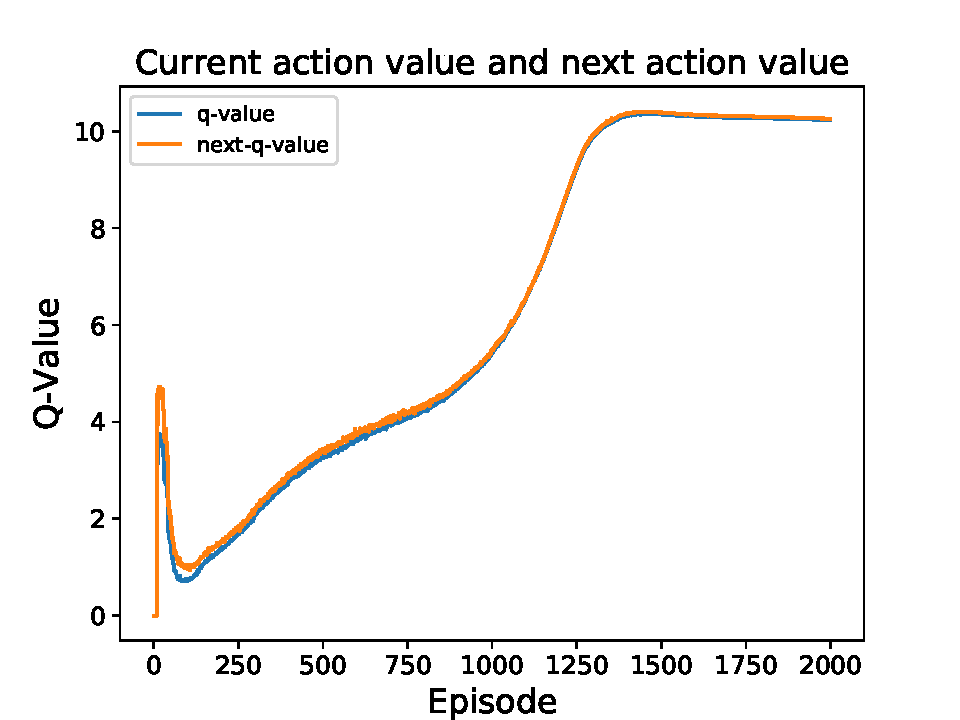
\includegraphics[width=2.5in]{cn2.pdf}
            }
            \subfloat[当前Q值与下一步的Q值之差的曲线]{
                \label{fig:dcn2}
                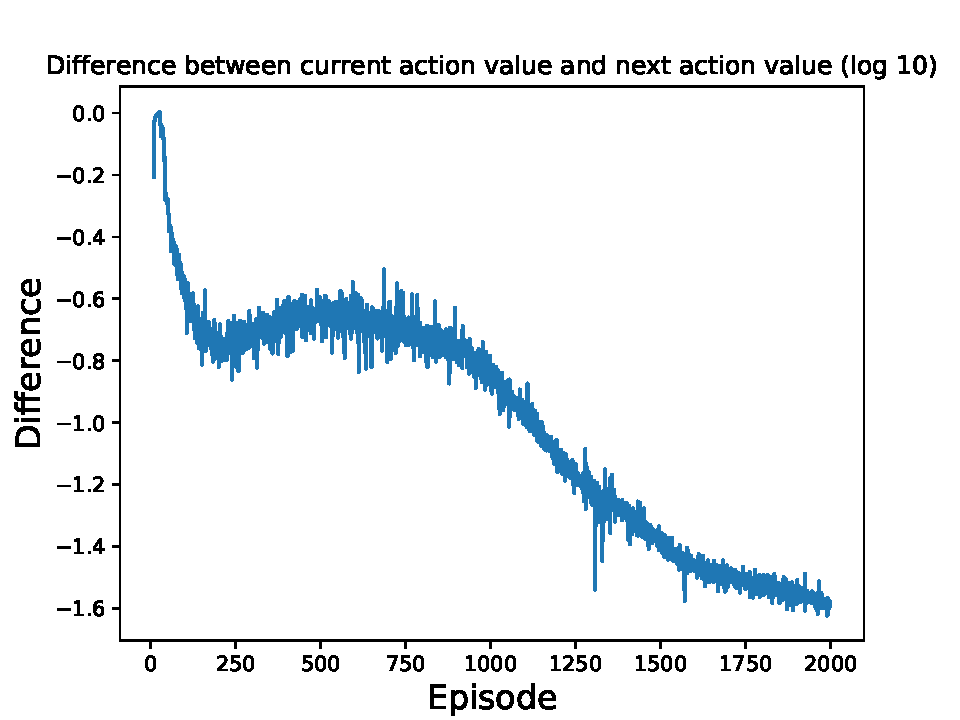
\includegraphics[width=2.5in]{dcn2.pdf}
            }
            \caption{当前Q值与下一步的Q值的相关曲线}
        \end{figure}        

        \begin{figure}[htb]
            \centering
            \subfloat[正确动作与错误动作的Q值曲线]{
                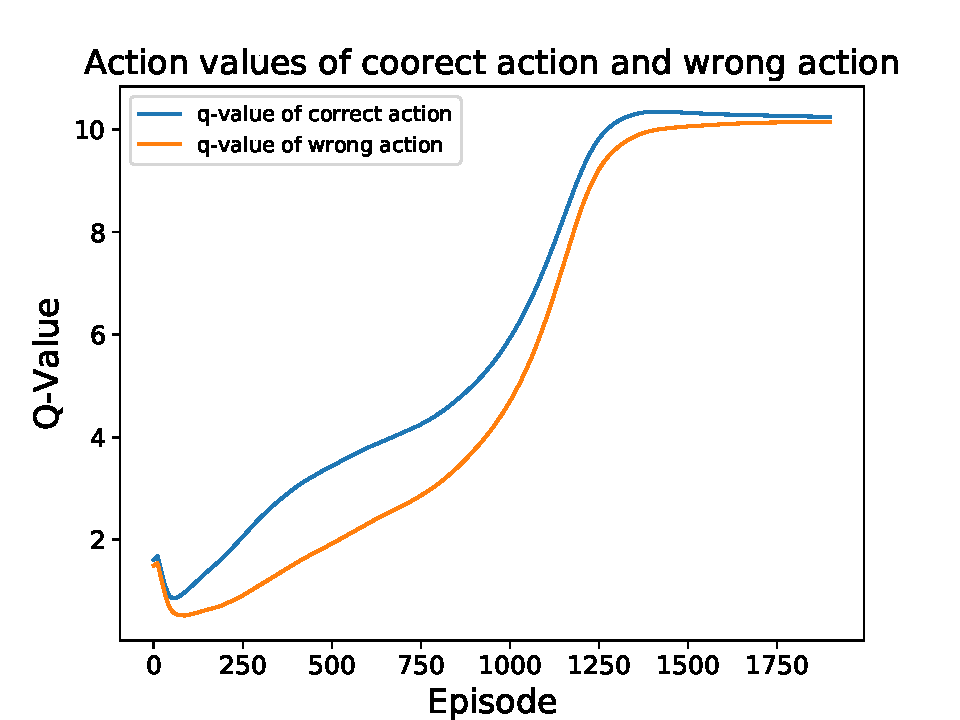
\includegraphics[width=2.5in]{cw2.pdf}
                \label{fig:cw2}
            }
            \subfloat[正确动作与错误动作的Q值之差的曲线]{
                \label{fig:dcw2}
                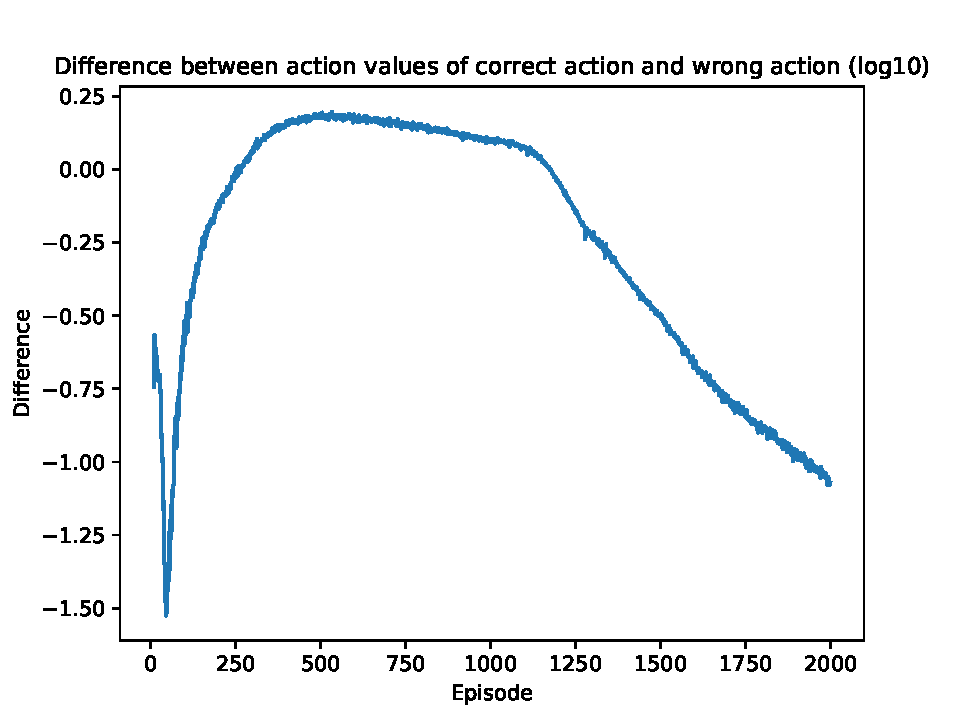
\includegraphics[width=2.5in]{dcw2.pdf}
            }       
            \caption{正确动作与错误动作的Q值相关曲线}
        \end{figure}
    \clearpage
    \section{总结}
        本文研究了DQN算法在CartPole问题上的应用,并对训练过程中产生的问题进行了一定的分析。通过分析,我们认为连续状态空间对于DQN算法来说需要一定的处理才可以发挥出更好的效果,如状态放大。

    
    \section{源码}
    环境要求:pytorch, gym, numpy, matplotlib
    \inputpython{main.py}{1}{334}
\end{document}